\chapter{The Access Control}

\section{Introduction}
The main tasks of the security system will be to ensure proper access
for the users and protect the structure and the content of any APIIS
databases from the unauthorised actions. 

APIIS needs guarantees that the persons connecting to the system
are really the ones they claim to be and also has to control the actions
each person is trying to perform. 


\section{Requirements for the access control system }

The requirements for the APIIS security system are split on three parts:

\begin{itemize}
\item general requirements
\item software requirements
\item database requirements
\end{itemize}

\subsection{General requirements \label{generalrequirements}}
\begin{itemize}
\item access to the APIIS System is controlled by the login and the password
\item access rights control is based on the RBAC\footnote{Role Based Access Control [2],[3]}(shortly saying the access rights are write down as a policies and the policies are assign to the roles)
\item access rights are granted to users through the role groups 
\item role group consist of the roles or other role groups
\item assigning users to the groups, group to the other groups or roles to the groups is controlled by the special constraints which are defined by the administrator (to prevent a situation where two excluding definitions are set together)   
\end{itemize}
\subsection{Software requirements\label{strequirements}}
\begin{itemize}
\item all APIIS software is placed in the secure space on the server - administrator account
\item developers have full access to the APIIS file system
\item normal users have access to read for the the APIIS file system 
\item all applications which cause modifications in the database (f.e. batch jobs) are restricted by the access rights
\item accessing the graphical interface, form tools, report tools is verified by defined access rights  

\end{itemize}
\subsection{Database requirements\label{dbtrequirements}}
\begin{itemize}
\item database is created and controlled by the administrator
\item users have not direct access into the database
\item access rights to the database granted by the administrator (for all users)
\item creating new database and new user is allowed only for the administrator
\item actions on the database objects like creating, altering, drooping are revoked from the users
\item access rights are specified for each table, column and the content of the column (record)  
\item operations on data like insert, update, delete and select are verified by the user access rights 
\item direct operations on data like insert, update, delete are not allowed for the user
\item all modifications on data carried through the administrator
\item selecting data permitted for the user through the views created by the administrator
\end{itemize}

%%%%%%%%%%%%%%%%%%%%% END SECTION - Requirements %%%%%%%%%%%%%%%%%%%%%%%%%%%%%%%%


%%%%%%%%%%%%%%%%%%%%% SECTION - The basic foundations %%%%%%%%%%%%%%%%%%%%%%%%%%%

\section{The basic foundations - setting APIIS software\label{settingapiis}}

\subsection{System architecture\label{systemarchitecture}}
There are three logical machines in an APIIS database setup: 
\begin{itemize}
\item client machine - the machine at which users operate
\item APIIS server - the machine that all users connect to
\item Database server - the machine that runs the backend database
\end{itemize} 
Clearly, all three logical machines can reside on one or more physical computers.\\
The client machine is the computer from where user fire up the web browser or just connect to the APIIS Server via SSH protocol\footnote{Secure Shell [4]}.\\
The APIIS Server takes care of the authentication of the users, connections to the database server and presenting data back to the users. Thus, to work directly on the APIIS server (via SSH), user must have an account on operating system level (see section \ref{registeringuseronOSL}) and also account on the APIIS system level (see section \ref{registeringuseronAPIISL}). The work with the web browser required only this second type of account.\\
The database server is the place where the database is stored. The connections into the database are supported by the APIIS Server. The connections to the database are distinguished on two groups: modifications on data and reading data. The modifications are executed only through the meta\_user connection (see \ref{apiisprojects}). Reading data is handled by the direct user connection.


\subsection{APIIS core\label{apiiscore}}

APIIS core software resides on the APIIS Server and is used by the all users. This means that programs are executed on the server and all users use the same libraries and modules.\\
Definition of security for the APIIS software is based on the usage some secure space on the server and also on the operating system features\footnote{The setup described here should be fullfiled during software installation}. Secure space is received by creating a special administrator account (OS account). Administrator is the owner of the files and this means that he has full rights to reading, writing and executing. Access to these files for the other users is handled by the special groups (see description of Linux groups). Each file has defined group to which belong and a special rights for this group (reading, writing and executing). In this case all files are defined in the administrator group (group is created with the administrator user account). This group can be ascribed to each operating system user and with this group user should have rights only to reading. If some of the files have to be fully restricted for the users (some administrator modules) than this can be done by removing all rights from the group and from the other users. In such case only administrator has access to these files.\\
There is also possibility to install separate copy of APIIS software for each user. In such case users must have operating system account because the software is installed in his home directory.
\bigskip 

\subsection{APIIS projects \label{apiisprojects}}
All projects based on the APIIS core have separate databases. In each of these database we have to create the meta\_user account. Then the PUBLIC schema has to be removed and the database must be created in the meta\_user schema\protect\footnote{Schema is essentially a namespace which contains named objects like tables, views whose names duplicates those of other objects existing in other schema's (PostgreSQL [1]).} which is created with the meta\_user account. In result the meta\_user has full access right to the database and only he can make direct modifications on the database content.
The important thing is that the meta\_user name have to be exactly the same like the name of the user defined in the model\_file of particular project.  There is only one model\_file for all users registered in the project.

The general schema how the system is implemented is shown on Figure \ref{fig:generalschema}.
\begin{figure}[h]
\begin{center}
   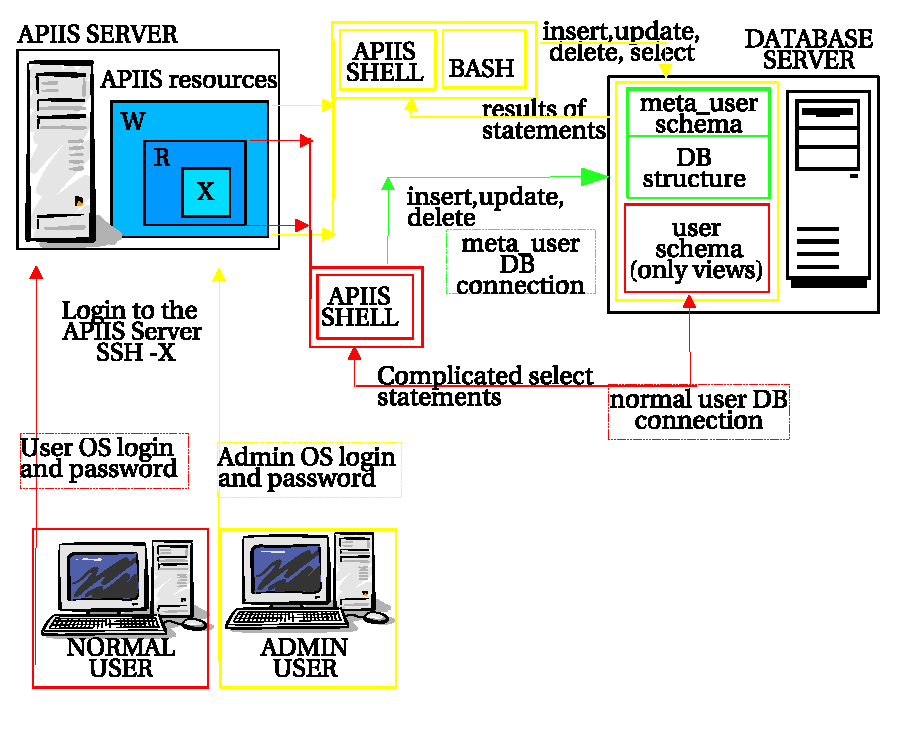
\includegraphics[scale=1]{./access-control/generalschema.eps}
   \caption{General schema for the access control system}
   \label{fig:generalschema}
\end{center}
\end{figure}
%%%%%%%%%%%%%%%%%%%%% END - The basic foundations %%%%%%%%%%%%%%%%%%%%%%%%%%%%%%%%%%%%%%%%


%%%%%%%%%%%%%%%%%%%%% SECTION - Defining users %%%%%%%%%%%%%%%%%%%%%%%%%%%%%%%%%%%%
\section{Defining users \label{definitionofuser}}
Only registered users can work in the system. Each user can be registered in the system on the two levels: 
\begin{itemize}
\item operating system level (not required for the each user),
\item APIIS system level (required for the each user. 
\end{itemize} 
 
\subsection{Registering user on the operating system level \label{registeringuseronOSL}}
This type of account is needed to work directly on the APIIS Server and it is related only to this users, which use the APIIS Shell or run some batch jobs. In such case user must have an account (login and password) in the operating system of APIIS Server.\\
Standard Linux user account can by created by executing the following command:
\begin{verbatim}
adduser [login] -g [login] -G [APIIS administrator group] 
\end{verbatim} 
During creation of account, the user is also assigned to the required Linux group (see \ref{apiiscore}).

At the end user APIIS\_HOME path have to be defined in .bash or .profile file. Path have to be redirected to the APIIS administrator space where the software is kept (see \ref{apiiscore}).
\begin{verbatim}
Example:
export APIIS_HOME=/home/apiis_administrator/devel/apiis
\end{verbatim} 

\subsection{Registering user on the APIIS system level \label{registeringuseronAPIISL}}
General APIIS account which is created on this level is required to work with the APIIS System. On the basis of this account the access rights for the user are created and then checked. The data about user are stored in the database (see section \ref{erddiagrams}, figure \ref{fig:users-groups-roles}: AR\_Users). The following information about each user is collected:
\begin{itemize}
\item login
\item password
\item db\_unit - foreign key to the unit table where the personal information about user is stored
\item country
\item language
\item marker - the information about the ownerschip of the data
\item disabled - this column is used to the locking of the user account. The flag of this column is always checked during the logging process and it can be set as YES (user can not login to the system) or NO (user can login to the system). There is also possibility to lock more then one user in the same time. This can be done by the lock of the user group to which the users are assigned
\item status, last\_login, last\_activ\_time - these three columns are used to controlling the user login time and to checking the user current status (see section \ref{furtherdevchecking}).
\end{itemize}

As an example of the user data, you can see Table \ref{usertable}.\\
\newpage 

\begin{table}[h]
\begin{center}\begin{tabular}{|c|c|c|c|c|c|c|}
\hline 
user\_id&login&password&db\_unit&country&language&marker\tabularnewline
\hline
\hline
1&kloss&******&22&German&DE\tabularnewline
\hline 
2&jkowal&******&455&Poland&Polish&PL\tabularnewline
\hline 
\end{tabular}\end{center}

\begin{center}\begin{tabular}{|c|c|c|c|}
\hline 
disables&status&last\_login&last\_activ\_time\tabularnewline
\hline
\hline
NO&ACTIVE&2005-07-29 09:38:28&2005-07-29 11:12:45\tabularnewline
\hline 
YES&INACTIVE&2005-05-12 11:12:45&2005-05-12 12:12:45\tabularnewline
\hline 
\end{tabular}\end{center}
\caption{Users table} \label{usertable}
\end{table}

The APIIS system is based on the PostgreSQL database and to work with it user needs also database account. PostgreSQL account is created automatically during the creation of APIIS account. The login and the password are exactly the same like these defined for the APIIS account.
This database account is needed for log-in to the system and also to give user the possibility of executing SQL SELECTs. These SELECT statements are executed on the views\footnote{The view is, in essence, a virtual table. It does not physically exist. Rather, it is created by a query joining one or more tables.} which are created in the user schema on the basis of user access rights.
The actions like insert, update, delete are effected by the meta\_user (\ref{apiisprojects}). The meta\_user is responsible for all modifications in the database and nobody else can do this. When the user executes a DML, the connection to the database is established from the meta\_user. Real user name is used to check user access rights. Then the meta\_user run all processes if the user has authorisation for this action. Real user name is sent as a normal data for the meta fields (last\_change\_user).\\
All other actions like creating, dropping and altering some objects are revoked from the user (even after log-in in to database from the command line). The user can not also create new users and databases.
%%%%%%%%%%%%%%%%%%%%% END SECTION -  creating users %%%%%%%%%%%%%%%%%%%%%%%%%%%%%%%%%%%%

%%%%%%%%%%%%%%%%%%%%% SECTION - Granting access rights %%%%%%%%%%%%%%%%%%%%%%%%%%%%%%%%%%%%
\section{Granting access rights to the user \label{garntingartu}}
The access rights are granted to the user by the role groups. Each registered user should be assigned at least to the one group (f.e. own which is created during the registration process). The information about groups assigned to the users is stored in the database table (see section \ref{erddiagrams}, figure \ref{fig:users-groups-roles}: AR\_User\_Groups):\\
\begin{table}[h]
\begin{center}\begin{tabular}{|c|c|}
\hline 
user\_id&group\_id\tabularnewline
\hline
\hline
1&1\tabularnewline
\hline 
1&3\tabularnewline
\hline 
\end{tabular}\end{center}
\caption{Relations beetwen users and groups} \label{usersgroupsrel}
\end{table}
\\group\_id is a foreign key to the group's table where the group definitions are stored (see section \ref{erddiagrams}, figure \ref{fig:users-groups-roles}: AR\_Groups table).
\begin{table}[h]
\begin{center}\begin{tabular}{|c|c|c|c|c|}
\hline 
group\_id&group\_name&group\_type&group\_content&group\_desc\tabularnewline
\hline
\hline
1&system\_task\_administrator&st\_group&Roles&description\tabularnewline
\hline 
2&database\_administrator&dbt\_group&Roles&description\tabularnewline
\hline 
3&breeder&dbt\_group&Groups&description\tabularnewline
\hline
\end{tabular}\end{center}
\caption{Groups} \label{grantinggroups}
\end{table}

The user is allocated for the group by the administrator. If the administrator wants to add the user to the group, first he has to check that the user can be really assigned to this group - checking that the group can cooperate with the groups which are currently defined for this user. This process is done automatically on the basis of the group constraints. The group constraints qualify which groups can not be used in the same time by the one user. They are stored in the separate table in the database (see section \ref{erddiagrams}, figure \ref{fig:constraints}: AR\_Group\_Constraints).\\
\begin{table}[h]
\begin{center}\begin{tabular}{|c|c|c|c|}
\hline 
group\_cons\_id&group1\_id&group2\_id&group\_cons\_type\tabularnewline
\hline
\hline
1&2&3&user-group-cons\tabularnewline
\hline 
2&6&4&user-group-cons\tabularnewline
\hline 
\end{tabular}\end{center}
\caption{Group constraints} \label{groupconstraints}
\end{table}

The fields group1\_id and group2\_id in the table are foreign keys to the table groups (Table \ref{grantinggroups}).
The algorithm, which veryfies the groups, takes from the user the current list of his groups (from table \ref{usersgroupsrel}). The values from the list are set together one by one with the id of the new group which we want to add. Each couple of values is used as a condition for the WHERE clause in the following SQL statement:
\begin{center}\emph{SELECT group\_cons\_id FROM ar\_group\_constraints WHERE
((group1\_cons\_id='}\textbf{\emph{user\_defined\_group}}\emph{' and group2\_cons\_id='}\textbf{\emph{new\_group}}\emph{') or (group1\_cons\_id='}\textbf{\emph{new\_group}}\emph{' and group2\_cons\_id='}\textbf{\emph{user\_defined\_group}}\emph{'))} and (group\_cons\_type='\textbf{user-group-cons}')\end{center}

For each couple of groups one SELECT is executed. When all combination of groups are positively verified (no results for each combination) then the user can be appraised to the group. If there is a result then this means that the constraints are defined for this combination and the new role group can not be added to the current set of groups defined for the user. The algorithm is not stooped in this point and it just go through the all combinations. All results are collected and then they are showed to the administrator. The administrator has clear picture which groups are in the conflict with the new group.\\
The constraints for the groups are optional and it should be defined only if they are needful (the decision stay with the administrator). In the section \ref{definingconstraints} you can read how the constraints are defined.

%%%%%%%%%%%%%%%%%%%%% END - Granting ar %%%%%%%%%%%%%%%%%%%%%%%%%%%%%%%%%%%%

%%%%%%%%%%%%%%%%%%%%% SUBSECTION - ARC for the system tasks %%%%%%%%%%%%%%%%%%%%%%%%%%%%%%%%%%%%

\section{Access rights for the system tasks \label{acfst}} 
\subsection{Definitions of the access rights \label{definitionarST}} 

This access control definition is designed for the scripts, forms, reports, interface, subroutines and all other actions which are executed on the basis of APIIS software (I called these action as a system tasks). The administrator of the system has to be sure that the user runs only these tasks which are allowed for him. This means that every user has to have defined access rights for the each system task. The definition of the access rights is based on the roles - roles based system (RBAC\footnote{Role Based Access Control [2],[3]}). In this type of system each role is a definition of the group of the access rights. In the roles, the access rights are defined via policies. In our case each policy defines access to one system task. All roles are grouped and they are assigned to the user groups. The whole structure of access control for the system tasks is defined in the following manner: the policies are ascribed to the one or more roles, the roles are ascribed to the one or more role groups, the role groups are ascribed to the one or more user or to the next role groups.\\
The information about access rights needed to control system tasks is stored in the three following tables (see section \ref{erddiagrams}, figure \ref{fig:stpolicies}):
\begin{itemize}
\item roles table (AR\_Roles) - this table stores information about roles. The role definition is a set of role name and the role type where the role type can be defined as ST (System Task) or DBT (Database Task). In this case the role should be defined as a ST.

\begin{table}[h]
\begin{center}\begin{tabular}{|c|c|c|}
\hline 
role\_id&role\_name&role\_type\tabularnewline
\hline 
1&sys\_admin\_role&ST\tabularnewline
\hline 
2&public\_role&ST\tabularnewline
\hline 
3&db\_admin\_role&DBT\tabularnewline
\hline 
\end{tabular}\end{center}
\caption{Roles table} \label{rolestable}
\end{table}

\newpage

\item system task policies table (AR\_StPolicies) - this table stores information about system tasks. Each system task consist of the name and the category. The category of the system task can be defined as: program, www, form, report, action. 

\begin{center}%
\begin{table}[h]
\begin{center}\begin{tabular}{|c|c|c|}
\hline 
stpolicy\_id&stpolicy\_name&stpolicy\_type\tabularnewline
\hline
\hline 
1&runall\_ar.pl&program\tabularnewline
\hline 
2&enter data&www\tabularnewline
\hline 
3&add new user&action
\tabularnewline
\hline 
4&Number of animals in year 2004&report
\tabularnewline
\hline
\end{tabular}\end{center}
\caption{Policies for the system tasks} \label {STpoliciestable}
\end{table}
\end{center}

\item link table (AR\_Role\_StPolicies) - it joins roles with the policies together. 
\end{itemize}

\subsection{Checking of the access rights - logging to the system \label{checkingARST}}
There are two ways to work with the APIIS system:
\begin{itemize}
\item directly on the APIIS server (APIIS Shell, batch jobs)
\item through the web browser (WWW service). 
\end{itemize}

If user wants to work directly on the APIIS server first he has to connect via ssh to the server (OS login and password - see section \ref{registeringuseronOSL}). After log-in to the server, special APIIS Shell is activated for the user. In the APIIS Shell user has to choose a project name (to which he want to login) and enters his APIIS login and the password (see section \ref{registeringuseronAPIISL}). If the data are consistent then the meta\_user has to check the user access rights for the system task. The meta\_user log-in to the database (the internal system connection) and checks which tasks user can execute. The result of this checking are returned as a list of the allowed jobs. This list is loaded in to the APIIS Shell. Finally user has only these actions in the Shell to which he is in the right. 
The symbolic schema is shown on Figure \ref{fig:serverloging}.\\
There are users which can have possibility to run batch jobs from the command line. In such case after log-in to the APIIS Server via ssh APIIS Shell is not activated automatically. The procedure of checking access rights for the programs which are run directly from the command line is exactly the same like during log-in via APIIS Shell. Difference here is that the meta\_user checks access right only for the currently executed task.\\
Second variant to work with the APIIS is the web browser. Here instead of connection to the server user has to specify in his web browser the correct address to the APIIS internet page. Login procedure is exactly the same like for the APIIS Shell.\\

\begin{figure}[h]
\begin{center}
   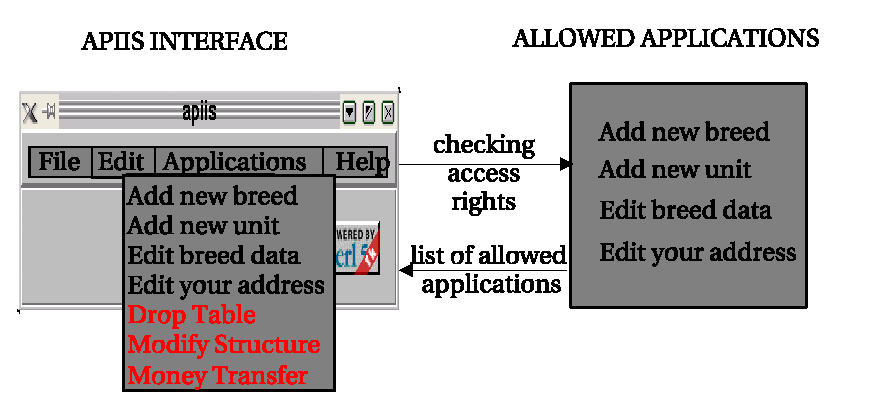
\includegraphics[scale=1]{./access-control/serverloging.eps}
   \caption{Logging to the APIIS system (red fields are not allowed)}
   \label{fig:serverloging}
\end{center}
\end{figure}
\newpage
%%%%%%%%%%%%%%%%%%%%% END SUBSECTION - AR for the sytem tasks %%%%%%%%%%%%%%%%%%%%%%%%%%%%%%%%


%%%%%%%%%%%%%%%%%%%%% SUBSECTION - ARC for the database  %%%%%%%%%%%%%%%%%%%%%%%%%%%%%%%%%%%%%%

\section{Access rights for the database and the content of the database \label{acfdb}}
This access control definition is designed for all action related to the database (database tasks).
We define two different methods for checking access rights on the database level. The choice of which,
depends on type of the SQL Statement.
One applies only to the \emph{insert, update and delete}
statements while another is used for the \emph{select} statements. The type of the SQL
Statement is recognised on the beginning and then the relevant method
is launched.

\subsection{Method for the insert, update and delete statements \label{insertupdatedelete}}

This route is especially for the insert, update, delete statements and can be described by the following steps: 
\begin{enumerate}
\item All actions go through the meta\_layer where the action is checked for the user
\item The arguments in the action (table/columns) are matched with the access
rights defined for this user,
\item If the user doesn't have required access rights for the table/columns
set the action is aborted, else access the record is checked in the next point. 
\item Algorithm checks if the statements will be executed on the set of data which are allowed for the user. If DML touches the record which is out of user area then the action is cancelled.
\end{enumerate}

\subsubsection{Definition of the access rights\label{definitionarDB}}

Definition of the access rights for the database tasks is based on the same structure like the definition of system tasks (\ref{definitionarST}). In this case access rights are also ordered by the roles where the role defines access rights to the group of tables, columns, records. The roles are assigned to the role groups. Each role consists of one or more policy. The policy consists of action (INSERT/UPDATE/DELETE), table name, column names for this table and the descriptor, where the descriptor specifies the sets of data on which user can operate. The information about access rights for the database tasks is also stored in the database (see section \ref{erddiagrams}, figure \ref{fig:dbt_policies}). In this case the same roles table which was defined for the system tasks is used (Table \ref{rolestable}). The difference is only in the role type definition because here the role is defined as a DBT (Database Task). Besides, there are three additional tables and the view:
\begin{itemize}
\item tables (AR\_DbtTables) - keeps information about the tables defined in the modelfile and their columns.

\begin{center}%
\begin{table}[h]
\begin{center}\begin{tabular}{|c|c|c|}
\hline 
table\_id&
table\_name&
table\_columns\tabularnewline
\hline
\hline 1  & breeds    & breed\_id|country\_id|lean\_meat\_avg	\\
\hline 2  & breeds    & breed\_id|tax\_id|mcname             	\\
\hline 3  & breeds    & breed\_id|lang\_id|intname           	\\
\hline 4  & animal    & db\_animal|birth\_dt|db\_sex|name    	\\
\hline 5  & breeds    & breed\_id|mcname|country\_id|tax\_id	\\
\hline 6  & breeds    & breed\_id|mcname			\\
\hline 7  & breeds    & breed\_id|mcname|tax\_id|dailygain	\\
\hline 8  & breeds    &	                 -                	\\ 
\hline 9  & animal    &	                 -                	\\ 
\hline
\end{tabular}\end{center}
\caption{Tables} \label{tables}
\end{table}
\end{center}

\item descriptor (AR\_DbtDescriptors) - table holds the definitions of filters for the reords. Descriptor can be defined as any column from the database. Each descriptor consist of the column name and the value for this column, where this last can be defined as a single value, list or range (range can be defined only for the numerical values). In case of list, there is a limitation related to the number of elements. If the list has more then 2000 elements then the special view in the user schema is created which will return values for this list. The name of this view is put in to the descriptor definition.\\
If the descriptor is based on the foreign key than the interanal representation of foreign key numbers is used as a values.
\begin{center}%
\begin{table}[h]
\begin{center}\begin{tabular}{|c|c|c|}
\hline descriptor\_id & descriptor\_name & descriptor\_value \\
\hline 
\hline 1  &  lean\_meat\_avg & 60-74	\\
\hline 2  &  tax\_id 	     & 5,6,7	\\
\hline 3  &  owner           & PL  	\\
\hline 4  &  db\_animal      & 1-50 	\\
\hline 5  &  db\_sex         & 72	\\
\hline 6  &  lean\_meat\_avg & 60-74 	\\
\hline 7  &  tax\_id         & 5,6,7 	\\
\hline 8  &  owner           & DE    	\\
\hline 9  &  db\_animal      & 1-10  	\\
\hline 10 &  db\_sex         & 72    	\\
\hline 11 &  tax\_id         & 1,2 	\\
\hline 12 &  carcassweight   & 300-400 	\\
\hline 13 &  owner           & PL,DE,FR,IT, ...\\
\hline 13 &  owner           & PL,DE	\\
\hline 14 &  owner           & FR 	\\
\hline 15 &  tax\_id         & 3 	\\
\hline 16 &  dailygain 	     & 24-56 	\\
\hline 17 &  NOT tax\_id     & 1,2,3 	\\
\hline
\end{tabular}\end{center}    
\caption{Descriptors}\label {descriptors}
\end{table}
\end{center}
 \newpage
\item database task policies - this table stores policy definitions which are a joins of records from tables: descriptor, table and codes. Table codes stores the SQL action names (1-INSERT, 2-UPDATE, 3-DELETE, 4-SELECT). The important thing is that the descriptor has to be always specified as a column of table which is used in the policy definition.

\begin{center}%
\begin{table}[h]
\begin{center}\begin{tabular}{|c|c|c|c|}
\hline 
policy\_id&action\_id&table\_id&descriptor\_id\tabularnewline
\hline
\hline 
1&1&1&1\tabularnewline
\hline 
2&1&2&2\tabularnewline
\hline 
3&1&3&3\tabularnewline
\hline 
4&1&4&4\tabularnewline
\hline
5&1&4&5\tabularnewline
\hline
6&2&1&1\tabularnewline
\hline 
7&2&2&2\tabularnewline
\hline 
8&2&3&3\tabularnewline
\hline 
9&2&4&4\tabularnewline
\hline
10&2&4&5\tabularnewline
\hline
11&3&8&2\tabularnewline
\hline
12&3&9&4\tabularnewline
\hline
13&4&5&11\tabularnewline
\hline
14&4&5&12\tabularnewline
\hline
15&4&5&13\tabularnewline
\hline
16&4&6&14\tabularnewline
\hline
17&4&6&15\tabularnewline
\hline
18&4&7&16\tabularnewline
\hline
19&4&7&17\tabularnewline
\hline
20&4&8&4\tabularnewline
\hline
21&4&8&5\tabularnewline
\hline
\end{tabular}\end{center}
\caption{Database task policies table}\label {dbpolicies}
\end{table}
\end{center}

\item user access view - the view is created in the user schema and keeps individual access rights of the user. The name of the view is derived from the user name.

\newpage
\begin{center}%
\begin{table}[h]
\begin{center}\begin{tabular}{|c|c|c|c|c|}
\hline 
action&tablename&columnames&descriptor\_name&descriptor\_value\tabularnewline
\hline
\hline insert & breeds & breed\_id|country\_id|lean\_meat\_avg		& lean\_meat\_avg 	& 60-74 \\
\hline insert & breeds & breed\_id|tax\_id|mcname 			& tax\_id 		& 5,6,7\\
\hline insert & breeds & breed\_id|lang\_id|intname 			& owner 		& PL\\
\hline insert & animal & db\_animal|birth\_dt|db\_sex|name 		& db\_animal 		& 1-10\\
\hline insert & animal & db\_animal|birth\_dt|db\_sex|name 		& db\_sex 		& 72\\
\hline update & breeds & breed\_id|country\_id|lean\_meat\_avg		& lean\_meat\_avg 	& 60-74   \\
\hline update & breeds & breed\_id|tax\_id|mcname			& tax\_id         	& 5,6,7    \\
\hline update & breeds & breed\_id|lang\_id|intname            		& owner           	& PL     \\
\hline update & animal & db\_animal|birth\_dt|db\_sex|name     		& db\_animal      	& 1-10   \\
\hline update & animal & db\_animal|birth\_dt|db\_sex|name      	& db\_sex        	& 72     \\
\hline delete & breeds & -						& tax\_id		& 5,6,7  \\
\hline delete & breeds & -						& db\_animal		& 1-50  \\
\hline select & breeds & breed\_id|mcname|country\_id|tax\_id 		& tax\_id 		& 1,2\\
\hline select & breeds & breed\_id|mcname|country\_id|tax\_id 		& carcassweight 	& 300-400\\
\hline select & breeds & breed\_id|mcname|country\_id|tax\_id 		& owner 		& PL,DE\\
\hline select & breeds & breed\_id|mcname 				& owner 		& FR\\
\hline select & breeds & breed\_id|mcname 				& tax\_id 		& 3\\
\hline select & breeds & breed\_id|mcname|tax\_id|dailygain 		& dailygain 		& 24-56\\
\hline select & breeds & breed\_id|mcname|tax\_id|dailygain 		& NOT tax\_id 		& 1,2,3\\
\hline select & animal & db\_animal|birth\_dt|db\_sex|name 		& db\_animal 		& 1-50\\
\hline select & animal & db\_animal|birth\_dt|db\_sex|name 		& db\_sex 		& 72\\
\hline
\end{tabular}\end{center}
\caption{User access rights view}\label{userarview}
\end{table}
\end{center}
 \end{itemize} 

\subsubsection{Checking of the access rights}

The procedure of checking access rights is executed for each SQL statement separately. Each SQL statement (from LO, forms, interface or 
other program), excluding SELECT, is parsed and the results are put into the special structure (record object). The information about SQL 
statement needed for the checking of access rights is taken from this structure.\\

\paragraph{\textbf{Checking insert statement}}

\begin{enumerate}
\item Getting the action name, table name and the column names from the SQL statement which user want to execute.
This information is taken from the record object.

\item Verifying user access rights for the action and the table.\\
Special ''SELECT'' statement is executed on the user access rights view. The action name and the table name (received in step 1) are used
as a arguments in the WHERE clause. It returns allowed column names and descriptors for defined table and action.\\
If there is some result from the SELECT statement then the access rights are valid for the action and the table and we can go to step 3. If there is no result (no record returned) user is not allowed to execute his SQL query and the algorithm is stopped.

\item Verifying user access rights for the columns.\\ 
Set of column from user SQL is matched with the sets of columns which are defined in the policies. If the algorithm finds the definition  which is identical (or if the policy definition contain all column from user SQL) then the descriptor of this policy is collected (the order of column can be different but the names have to be the same). Algorithm goes through the all records returned in step 2 and accumulates all descriptors. Error message (no access rights) is generated in case if there is no applicable column definitions in the user rights.

\item Verifying user access rights for the record .\\
Now we have to prove all descriptors returned in the previous step. The value of each descriptor is set together with the value of the corresponding column from the user SQL\footnote{if the descriptor value is defined as a list or range then the value from user SQL is searched on the list or it is collated with the range; in case of view the select statement is executed to verified this value.}. If the value from user SQL is in the right with the descriptor value then the next pair of value is checked. If there is no compatibility for some pair of value then the error message is printed and action is stopped. The process of access rights checking is finished successfully if data introduced by the insert are contained in the user limitations. 
\end{enumerate}
Examples:
\begin{center}
\begin{verbatim}
(1) INSERT INTO breeds(breed_id,country_id,lean_meat_avg)
      VALUE (50000055,500000001,68);
(2) INSERT INTO breeds(breed_id,country_id,lean_meat_avg)
      VALUE (50000055,500000001,45);
(3) INSERT INTO breeds(breed_id,tax_id)
      VALUE (50000055,6);
(4) INSERT INTO breeds(breed_id,country_id,tax_id,lean_meat_avg)
      VALUE (50000055,500000001,7,45);
(5) INSERT INTO breeds(breed_id,lang_id,intname)
      VALUE (50000055,300000001,'name');
\end{verbatim}
\end{center}
If we look at our view (Table \ref{userarview}) then: 
- the first insert can be executed by the user because the lean\_meat\_avg is 68  and allowed range is 60-74\\
- the second insert can not be executed because lean\_meat\_avg is out of defined range \\
- the third insert can be executed \\
- the forth insert can not be executed because there is no such set of column definitions in any policy.\\
- the fifth insert can be executed if the owner name which will be inserted to the record is defined as PL (the owner is a special case     which is existing only in EFABIS project and it is taken from the user table).  

\paragraph{\textbf{Checking update statement}}

The procedure of checking access rights for update is exactly the same like this defined for the insert. The differences are only in steps 2 and 4. In step 2, the parameter action for the WHERE caluse is defined as UPDATE. In step 4 descriptors are compared with the values of record which will be updated by the user (in the INSERT they are compared with the values which are introduced by the user).\\

Examples:
\begin{center}
\begin{verbatim}
(1) UPDATE breeds SET breed_id='50000045',mcname='new mcname'
      WHERE breed_id=444446;
(2) UPDATE animal SET birth_dt='2000-09-02', db_sex=73
      WHERE db_animal=444556;
(3) UPDATE animal SET birth_dt='2000-09-02', name='some name' 
      WHERE db_animal>1 and db_animal<10 and db_sex=73;
\end{verbatim}
\end{center}

In our examples the first update can be executed if the tax\_id of existing record is defined as 5 or 6 or 7. The second update can not be executed because db\_animal is out of the range. The third record can be also not executed because action is allowed only for the records where db\_sex has 72 value (in this case db\_animal is correct). 

\paragraph{\textbf{Checking delete statement}}
In case of DELETE statement the algorithm works the same like for UPDATE with exclusion of step 3 (DELETE statement is executed on the whole record and the columns are not checked).

The symbolic schema of modifying database content is shown on the Figure \ref{fig:modifingdata}.
\begin{figure}[h]
\begin{center}
   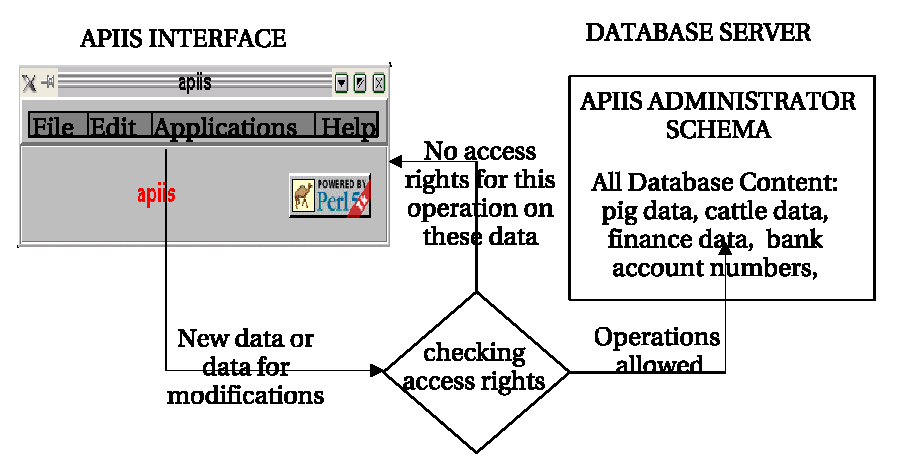
\includegraphics[scale=1]{./access-control/modifingdata.eps}
   \caption{Modifying the database content}
   \label{fig:modifingdata}
\end{center}
\end{figure}
\\All modifying query (insert,update,delete) are managed by the metauser (see \ref{databaselevel}).

\newpage

\subsection{Method for the public select statements\label{select}}

Access rights for the public SELECT statements follow a different route from the method
which was described in the previous section. This route is different, because the parsing of a complex SELECT statement (placing elements of the SQL query into the record object) is too complicated.
In this case SELECT statements are not handled by the meta\_user but by the real user with his direct database connection. They are executed on the views located in the user schema. User can access only these views which are created in his schema. Each view contains only those rows and columns that the user is allowed to access (on the basis of his access rights).

\subsubsection{Definition of the access rights:}
Access rights for the selecting data are defined in the same way like were defined for \emph{update,
insert} and \emph{delete} (see \ref{insertupdatedelete}).

\begin{center}%
\begin{table}[h]
\begin{center}\begin{tabular}{|c|c|c|c|c|}
\hline 
action&tablename&columnames&descriptor\_name&descriptor\_value\tabularnewline
\hline
\hline select & breeds & breed\_id|mcname|country\_id|tax\_id 		& tax\_id 		& 1,2\\
\hline select & breeds & breed\_id|mcname|country\_id|tax\_id 		& carcassweight 	& 300-400\\
\hline select & breeds & breed\_id|mcname|country\_id|tax\_id 		& owner 		& PL,DE\\
\hline select & breeds & breed\_id|mcname 				& owner 		& FR\\
\hline select & breeds & breed\_id|mcname 				& tax\_id 		& 3\\
\hline select & breeds & breed\_id|mcname|tax\_id|dailygain 		& dailygain 		& 24-56\\
\hline select & breeds & breed\_id|mcname|tax\_id|dailygain 		& NOT tax\_id 		& 1,2,3\\
\hline select & animal & db\_animal|birth\_dt|db\_sex|name 		& db\_animal 		& 1-50\\
\hline select & animal & db\_animal|birth\_dt|db\_sex|name 		& db\_sex 		& 72\\
\hline
\end{tabular}\end{center}
\caption{The same user access rights view}\label{userselectview}
\end{table}
\end{center}



\subsubsection{Creating views:}

Each user view is created separately. Always for each table one view is created. At the beginning list of all allowed
table names is taken from the user access rights view (only these table
names on which user can execute SELECT statement).

\begin{flushleft}Then the following steps have to be accomplished to create view for each table from the list:\end{flushleft}

\begin{enumerate}
\item Creating list of basic columns for the view.\\
The algorithm takes from the user access view all column names for the table which is currently treated. The column names are taken from the each policy definition and then they are merged together in to the one list (duplicates of columns are removed). This list is needed to create basic view structure.

\item Creating basic SQL statement needed to produce view.\\
This first part of the SQL statement is defined on the basis of the columns which we got in the previous step. 

\begin{center}\emph{CREATE VIEW} \textbf{\emph{user\_schema.treated\_table}}
\emph{AS SELECT} \textbf{\emph{list of basic columns}}
\emph{FROM meta\_user\_schema.treated\_table WHERE oid=NULL ......}\end{center}
The ''where clause'' is needed here to create empty view structure.
Now we have to add the filtration for the columns and the records according to the descriptor definitions. 


\item Defining filtering extensions for the basic SQL statement.\\
The records are filtered by the additionall SELECT statements which have to be defined separately for the each unique set of columns.  SELECTS are created one by one and for each of them the following actions are effected:
\begin{itemize}
\item At first the column for the SELECT are prepared. Treated set of columns is compared to the basic list from step 1. If some column is missing in the treated set then NULL expresion is placed instead of column. The order of column for this query has to be exactly the same like the order of basic column.
\item When the columns are ready then the WHERE clause is fixed. Thus all descriptors assigned for considered collection of columns have to be included. Each of the descriptors is joined to the WHERE clause by the AND operator. If descriptor has more than one value defined then the one condition from these values is created. In this case value are link by the OR operator\footnote{This is true only if we have a list of value, in case of the range values are merged by AND operator} and then they are added to the WHERE clause. It can be also that the value of descriptor is related to the view and then the information are taken by the additional subquery (construction: descriptor IN (SELECT) ).\\
If descriptor name is defined with the NOT prefix, the NOT expression is added to the WHERE before this element\footnote{NOT expression can help prevent views before duplicated records}.
\item The complete SELECT is added to the basic SQL statement (from step 2) by the UNION expression. After this the next set of columns is taken into the process.
\item After last SELECT finall SQL is executed and the view for the table is created.
\end{itemize}

Example:
\begin{verbatim}
CREATE VIEW user\_schema.breeds as 
    SELECT breed\_id, mcname, country\_id, tax\_id, dailygain FROM breeds
  UNION
    SELECT breed\_id, mcname, country\_id, tax\_id, NULL FROM breeds
      WHERE (tax\_id=1 or tax\_id=2) 
              and (carcassweight>=300 and carcassweight<=400)
                and (owner='PL' or owner='DE') 
  UNION
    SELECT breed\_id, mcname, NULL, NULL, NULL FROM breeds
      WHERE (owner='FR') and (tax\_id=3)
  UNION
    SELECT breed\_id, mcname, NULL, tax\_id, dailygain FROM breeds
      WHERE (dailygain>=24 and dailygain<=56) and not((tax\_id=1 and so on ...); 

\end{verbatim}
In result we get a following view:
\begin{center}
\begin{table}[h]
\begin{center}
\begin{tabular}{|c|c|c|c|c|}
\hline breed\_id & mcname & country\_id & tax\_id & dailygain\\
\hline
\hline 33 & Polish Red & 50000091 & 1 & NULL \\
\hline 45 & Angler     & 50000009 & 1 & NULL \\
\hline 67 & Wollschwein& 50000009 & 2 & NULL \\
\hline 56 & Pulawska   & 50000091 & 2 & NULL \\
\hline 23 & Duck de la France & NULL & NULL & NULL \\
\hline 78 & Lanka & NULL & 5 & 350 \\
\hline 24 & Florina & NULL & 6 & 315 \\
\hline
\end{tabular}
\end{center}
\caption{View for the breeds table} \label{breedviewexample}
\end{table}
\end{center}

The symbolic schema of reading data is shown on Figure \ref{fig:readingdata}.
\begin{figure}[h]
\begin{center}%
   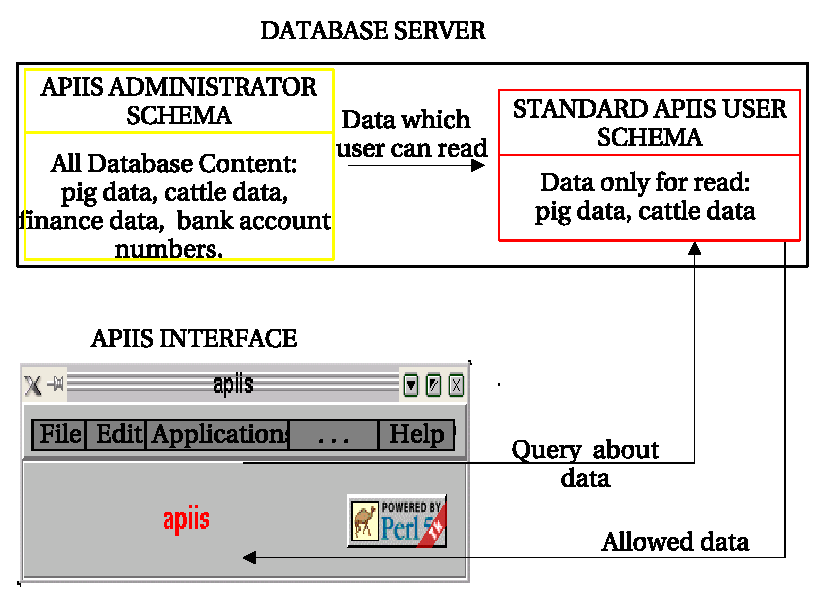
\includegraphics[scale=1]{./access-control/readingdata.eps}
   \caption{Reading data from the database}
   \label{fig:readingdata}
\end{center}
\end{figure}

\end{enumerate}

\section{Grouping access rights \label{groupingar}} 

All access rights in the system are granted to the user by the groups. The group is a bunch of access rights which can be assigned to the one or more user. Each group can be structured from roles or other groups. The important thing is that this two elements can not be mixed in the one group. The main role group definitions are kept in the database table (AR\_Groups)\footnote{The table was already presented in the section \ref{garntingartu}}.\\
\begin{table}[h]
\begin{center}\begin{tabular}{|c|c|c|c|c|}
\hline 
group\_id&group\_name&group\_type&group\_content&group\_desc\tabularnewline
\hline
\hline
1&system\_task\_administrator&st\_group&Roles&description\tabularnewline
\hline 
2&database\_administrator&dbt\_group&Roles&description\tabularnewline
\hline 
3&breeder&dbt\_group&Groups&description\tabularnewline
\hline
\end{tabular}\end{center}
\caption{Groups}\label{groupinggroups}
\end{table}
\newpage
\subsection{Grouping roles \label{groupingroles}} 
Each role is allocated at list in the one group. The relations beetwen the the roles and role groups are kept in the separate table (AR\_Role\_Groups). The role is allocated for the group by the administrator. If we want to add the role to some group, first we have to check the group type (the type of the role has to be the same type like the type of the group) and the group content (role can be added to the group which contains roles definition - not other groups). If these two requirements are agreed then we have to investigate that the new role can cooperate with the other roles which are currently defined in this group. This process is done automatically on the basis of the role constraints defined for the roles. These constraints qualify which roles can not be used in the same time in the one role group. The constraints for the roles are stored in the different table (see section \ref{erddiagrams}, figure \ref{fig:constraints}): AR\_Role\_Constraints) than the constraints for the groups (see section \ref{erddiagrams}, figure \ref{fig:constraints}): AR\_Group\_Constraints).
\begin{table}[h]
\begin{center}\begin{tabular}{|c|c|c|}
\hline 
role\_cons\_id&role1\_cons\_id&role2\_cons\_id\tabularnewline
\hline
\hline
1&1&2\tabularnewline
\hline 
\end{tabular}\end{center}
\caption{Constraints for the roles}\label{brr}
\end{table}

The fields role1\_id and role2\_id are foreign keys to the roles table (AR\_Roles table). 
The algorithm, which veryfies the roles, takes from the group (to which we want to add the role) the current list of its roles. The values from the list are set together one by one with the id of the new role. Each couple of values is used as a condition for the WHERE clause in the following SQL statement:
\begin{center}\emph{SELECT role\_cons\_id FROM ar\_role\_constraints WHERE
(role1\_cons\_id='}\textbf{\emph{existing\_role}}\emph{' and role2\_cons\_id='}\textbf{\emph{new\_role}}\emph{') or (role1\_cons\_id='}\textbf{\emph{new\_role}}\emph{' and role2\_cons\_id='}\textbf{\emph{existing\_role}}\emph{')}\end{center}

For each couple of roles one SELECT is executed. When all combination of roles are positively verified (no results for each combination) then the role can be appraised to the group. If there is a result for some union then this means that there are some constraints and role can not be added to the group. The algorithm is not stooped in this point and it just go through the all combinations. All results are collected and then they are showed to the administrator. The administrator has clear picture which roles are in the conflict with the new role.

\subsection{Grouping groups \label{groupinggroups}} 
The groups can be also assigned to the other groups. This can be done only if the content of the group to which we want to add new group is defined as "Groups" and the types of the groups are the same. The relations beetwen the groups are kept in the separate database table (see section \ref{erddiagrams}, figure \ref{fig:users-groups-roles}): AR\_Group\_Groups) where we define the group\_id from higher level (parent) and group\_id from lower level (child). In this table the unique key is defined on both of the columns. The important rules are that the group can not be ascended to itself and also that there is no possibility to create the same combination of groups but with different order of columns (the group ids changed beetwen the columns).\\
If we want to add the group to the other group, we have to be in right with the condition presented above. Then we have to check the group constraints (checking that the new child group can cooperate with the other already defined child groups).  This constraints are stored in the same table where the constraints for the assigning user to the groups are defined (AR\_Group\_Constraints - Table \ref{groupconstraints}). The difference is only in the relation type, her it is defined as "group-group".

In this case the algorithm takes from the parent group the current list of its child groups. The existing children are set together one by one with the new child. Each couple of values is used as a condition for the WHERE clause in the following SQL statement:
\begin{center}\emph{SELECT group\_cons\_id FROM ar\_group\_constraints WHERE
((group1\_cons\_id='}\textbf{\emph{existing\_child\_group}}\emph{' and group2\_cons\_id='}\textbf{\emph{new\_child\_group}}\emph{') or (group1\_cons\_id='}\textbf{\emph{new\_child\_group}}\emph{' and group2\_cons\_id='}\textbf{\emph{existing\_child\_group}}\emph{'))} and (group\_cons\_type='\textbf{group-group-cons}')\end{center}

For each couple of role values one SELECT is executed. When all combination are positively verified (no results for each combination) then new child group can be appraised to the parent group. If there is a result for some union then this means that some constraints are defined and new group can not be added. The algorithm is not stooped in this point and it just go through the all combinations. All results are collected and then they are showed to the administrator. The administrator has clear picture which existing groups are in the conflict with the new child group.\\

\section{Specifying constraints for the grouping\label{definingconstraints}} 
In the previous sections we specified the three types of constraints which are use in the grouping:
\begin{enumerate}
\item user-groups-constraints - checking if the user can be ascribed to the new group with his current aggregation of groups
\item group-groups-constraints - checking if the group can be defined as a part of other group.
\item role-constraints - checking if the role can be added to the group
\end{enumerate}
The manner of adding new constraints for each of this category is very similar. At the beginning we have to check that the new constraints will be valid for the current definitions allocated for the user and groups (f.e. one of the user is assigned to two groups which we want to exclude). Thus the one of the following statements have to be executed:\\
\begin{center}
\emph{SELECT user\_id FROM ar\_user\_groups WHERE
group\_id='}\textbf{\emph{first group id}}\emph{' or group\_id='}\textbf{\emph{second group id}}
\end{center}
This SELECT is executed for the first type of constraints. In the WHERE clause we put these group ids for which the new constraint will be defined. As a result we get a users which are attributed for these groups.\\ 

\begin{center}
\emph{SELECT hl\_group\_id FROM ar\_group\_groups WHERE
ll\_group\_id='}\textbf{\emph{first group id}}\emph{' or ll\_group\_id='}\textbf{\emph{second group id}}
\end{center}
The SELECT is executed for second type of constraints. In the WHERE clause we put these group ids for which we want to define new constraint. SELECT returns these parent groups which have such child groups defined.\\
 
\begin{center}
\emph{SELECT group\_id FROM ar\_role\_groups WHERE
role\_id='}\textbf{\emph{first role id}}\emph{' or role\_id='}\textbf{\emph{second role id}}
\end{center}
The last SELECT is executed for the third type of constraints. In the WHERE we put the role\_id for which we want to define new constraint. Returned results give the information about groups to which these roles are assigned.\\

After this when the SELECT is executed, the algorithm checks if there are any duplicates in the returned results (two the same user, two the same groups). If the duplicates are presented  for one of this SELECT then they are returned as an one conflicts list. In such case the new constraints can not be added because it causes a contradiction in the current definitions. The administrator first has to change these conflict definitions and then this constraints can be introduced.
\newpage
\section{Further developing\label{furtherdev}}

\subsection{Checking the login time and the current status of the users\label{furtherdevchecking}}
The method of checking the login time for the user is needed to prevent system before unclosed session. There are three columns in the users table which are used by this method: session\_status column which is fill in during the logging (the flag of this column is set as ACTIVE), last\_login column which is fill in by the logging timestamp and last\_activ\_time column which is updated during the user session. The last column is updated by the actual timestamp everytime when the user executes some action on the database. In the same time algorithm checks also the activation time for the all others users and compares it with the actual time. If the difference for some user is greater then defined timeout then the user session is closed. The timeout should be defined as a global value in the configuration file.

\section{Remarks}
Implementation of the Security System is made in the Perl Programming Language. 

\section{Bibliography}
\begin{verbatim}
[1] http://www.postgresql.org/docs/7.4/static/sql-createschema.html 
[2] David F. Ferraiolo, Ravi Sandhu, Serban Gavrila, D. Richard Kuhn,
    Ramaswamy Chandramouli, 
    Proposed NIST Standard for Role-Based Access Control, (ACM, 2001) 
[3] http://csrc.nist.gov/rbac/
[4] http://en.wikipedia.org/wiki/SSH
\end{verbatim} 

\section{ERD diagrams\label{erddiagrams}}

\begin{figure}
\begin{center}%
   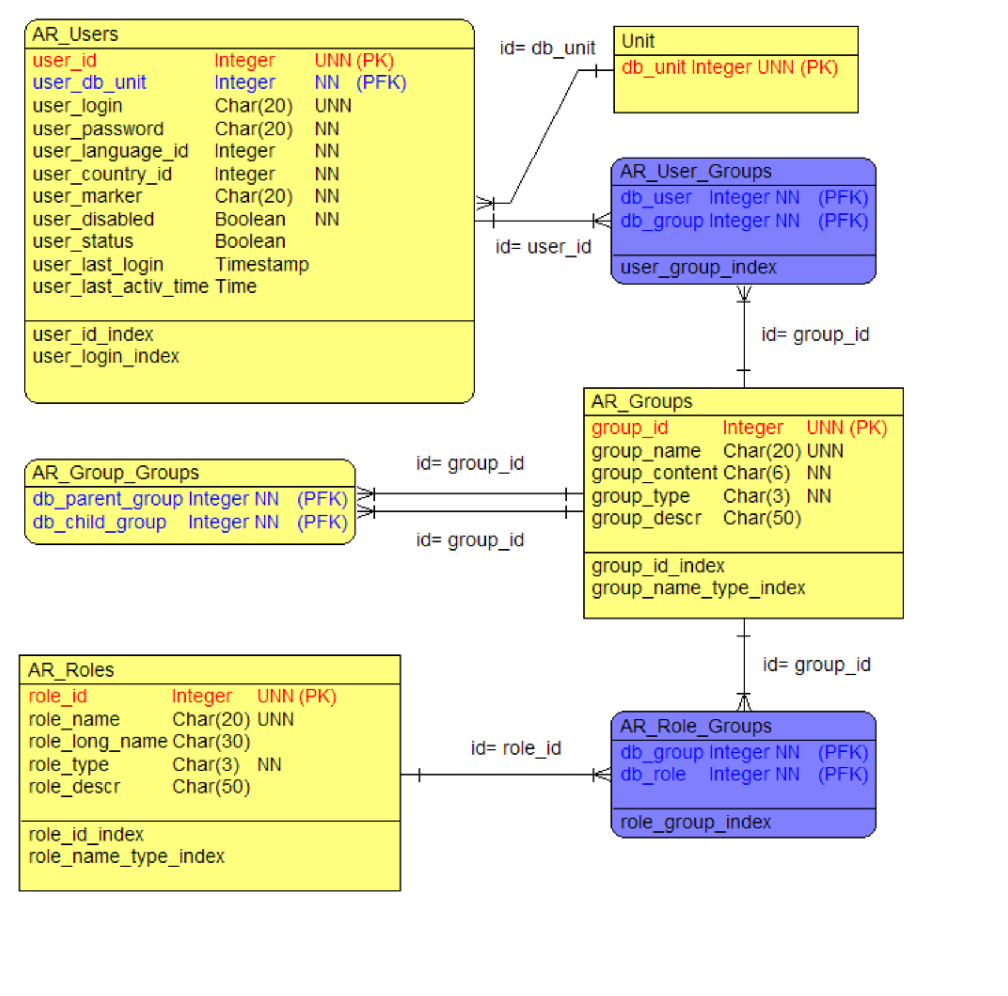
\includegraphics[scale=1]{./access-control/ar_user_group_role.eps}
   \caption{Users-Groups-Roles}
   \label{fig:users-groups-roles}
\end{center}
\end{figure}

\begin{figure}
\begin{center}%
   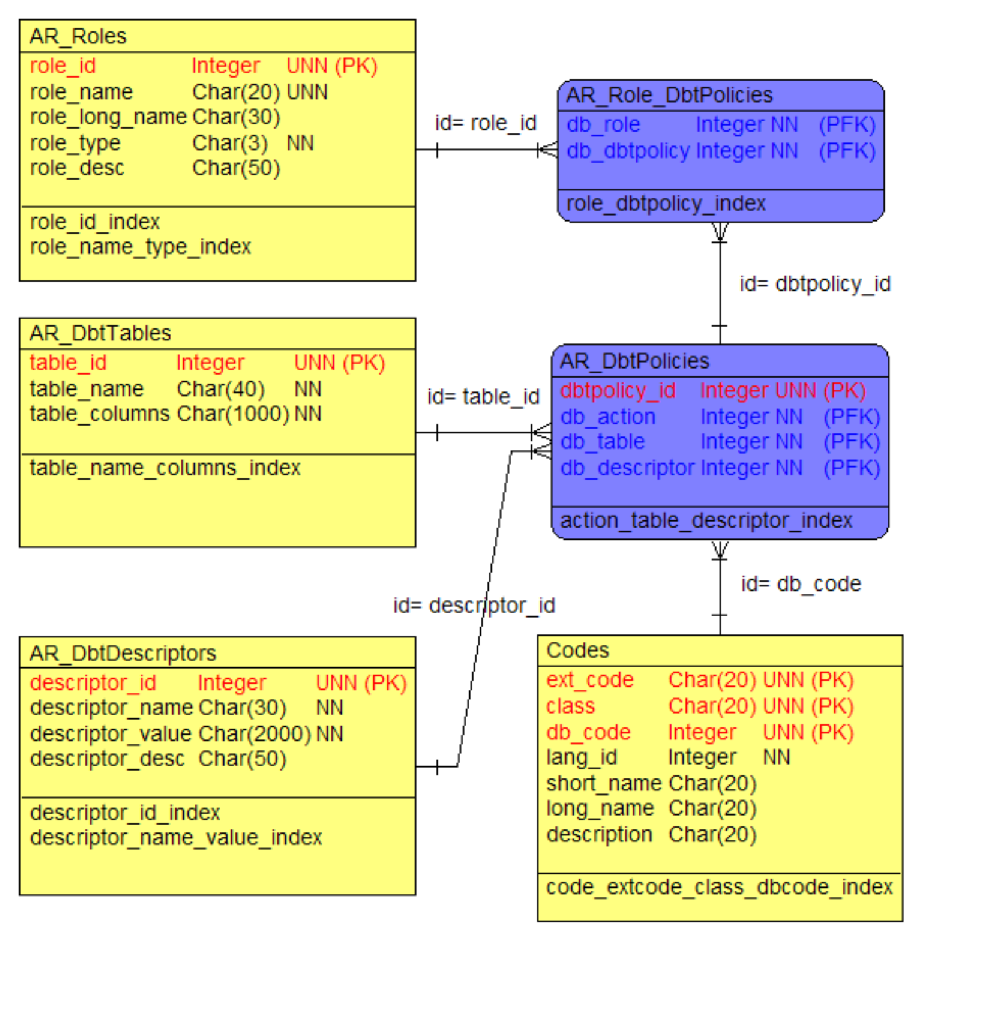
\includegraphics[scale=1]{./access-control/ar_dbtpolicies.eps}
   \caption{Access rights for the database tasks}
   \label{fig:dbt_policies}
\end{center}
\end{figure}

\begin{figure}
\begin{center}%
   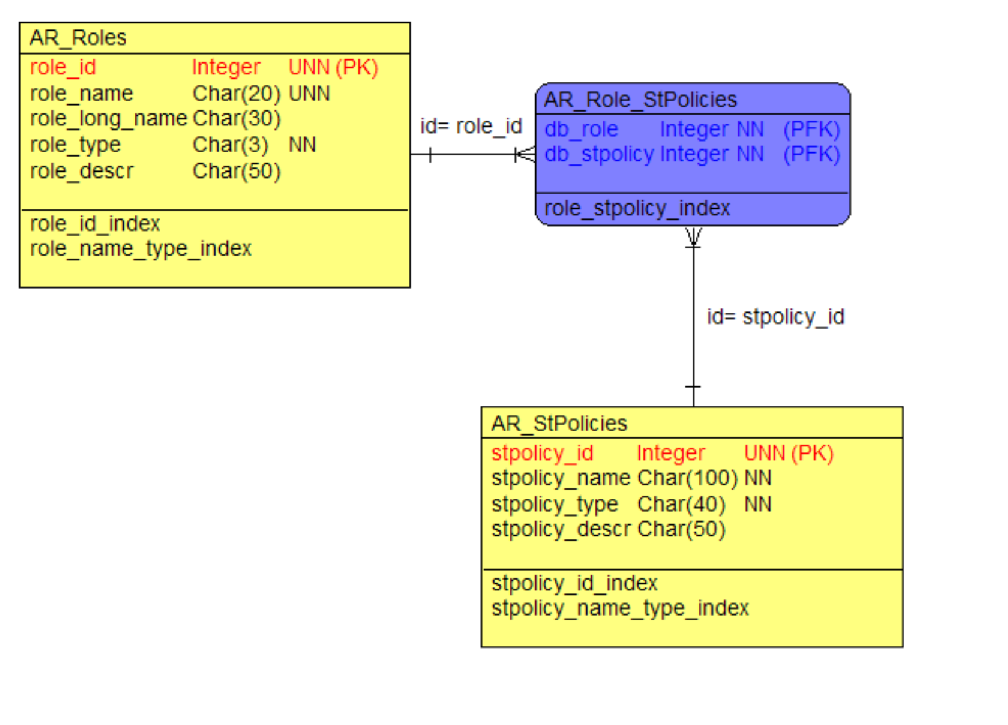
\includegraphics[scale=1]{./access-control/ar_stpolicies.eps}
   \caption{Access rights for the system tasks}
   \label{fig:stpolicies}
\end{center}
\end{figure}

\begin{figure}
\begin{center}%
   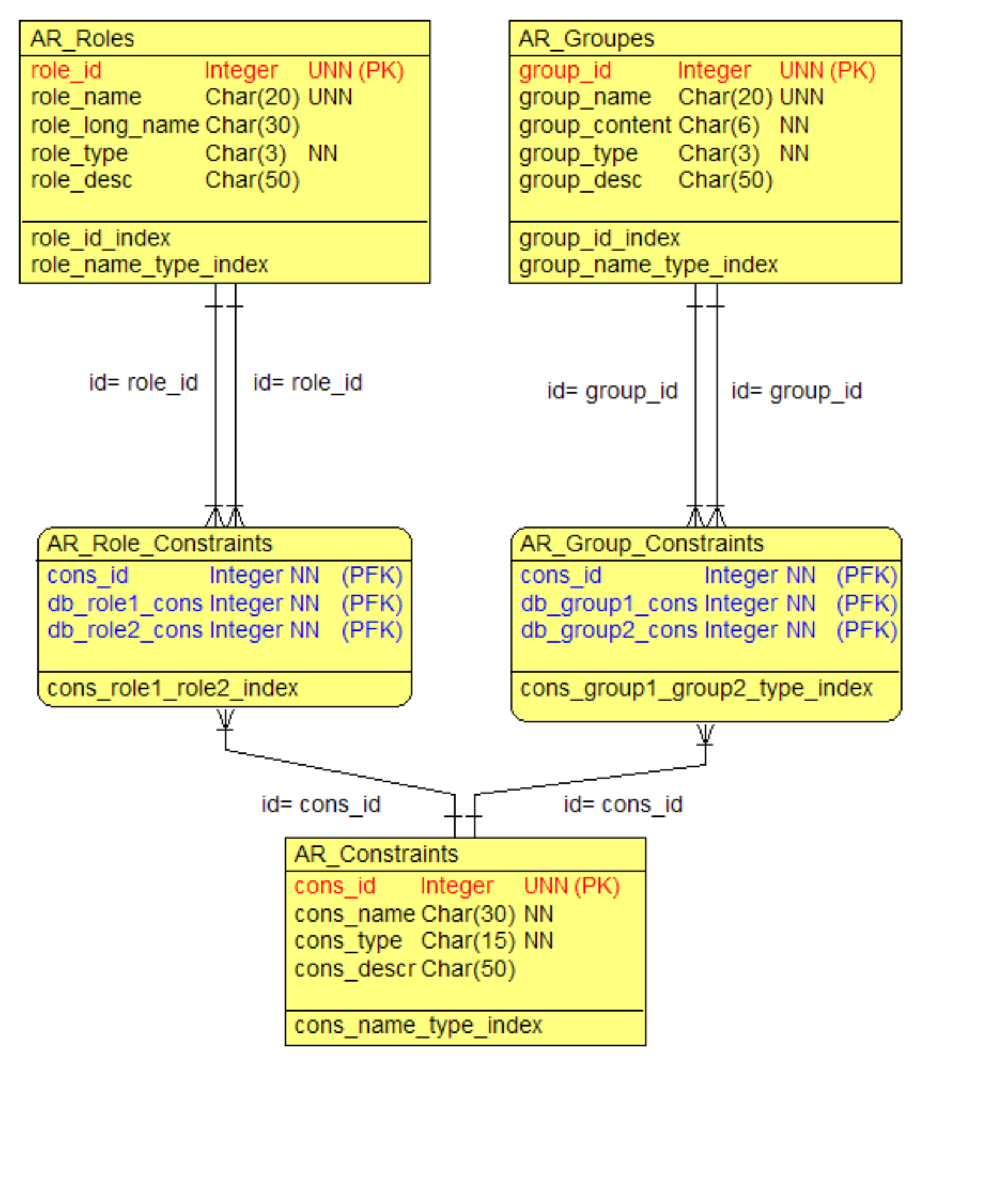
\includegraphics[scale=1]{./access-control/ar_constraints.eps}
   \caption{Constraints}
   \label{fig:constraints}
\end{center}
\end{figure}

